\documentclass[notitlepage]{article}
\usepackage{ctex}
\usepackage{graphicx}
\usepackage[a4paper, scale=0.85]{geometry}

\title{心得体会}
\author{}
\date{}

\setlength{\parindent}{2em}
\linespread{2}

\begin{document}

\maketitle

\vspace{-4em}

本次实验增进了我对模式识别课程的知识的理解,同时让我更加熟悉基于python的机器学习
库scikit-learn以及深度学习库pytorch的使用,并且提升了我的编程能力。

值得注意的是,本次实验的实验二——KNN分类任务中关于NCA算法的阐释上存在严重的错误,
原实验说明文档中提到的是最小化同类样本相似程度,但实际上应当是最大化,具体的推导
过程见实验报告中实验二部分

\begin{figure*}[htbp]
    \centering
    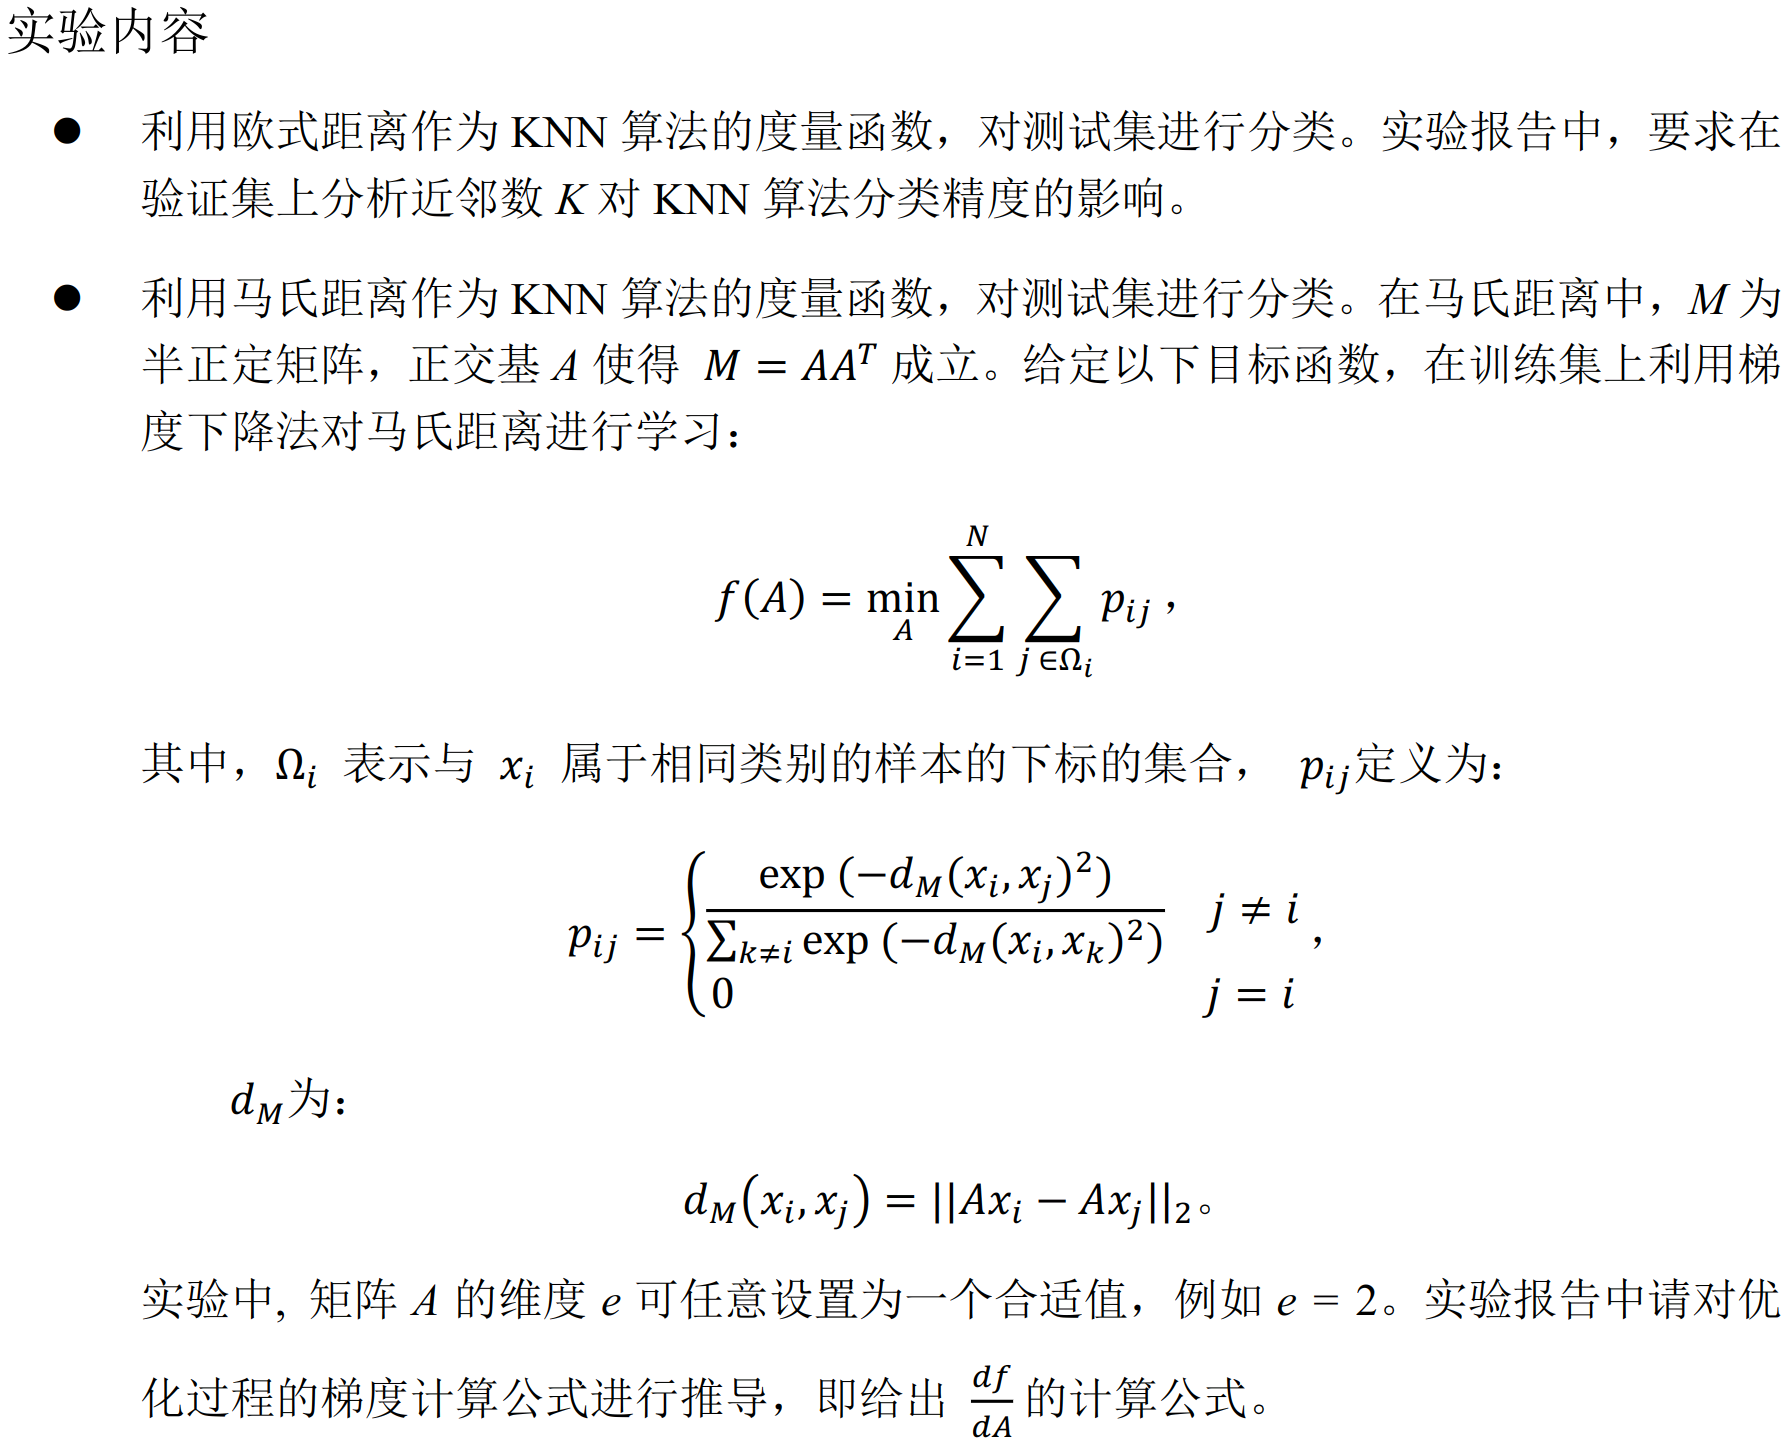
\includegraphics[width=\columnwidth]{imgs/nca.png}
    \caption{实验文档中对于NCA算法的表述}
\end{figure*}

\end{document}